\chapter{State-of-the-art} \label{chap:State_of_the_art}

In the present chapter, a review of the current technology related to the topic of this work will be reviewed. Firstly, a review of the different morphing wing technologies will be introduced. Secondly, a particular focus on the state-of-the-art of technology exploit in the current project will be presented.

\section{Morphing aircraft} \label{sec:Morphing_state}

The interest in morphing of the aerodynamic surfaces has accompany aerospace history since the beginning. Since the first heavier-than-air flight in 1903, when the Wright Brothers designed and build the first controlled, sustained flight of a powered heavier-than-air aircraft. Their concept of aircraft did not provide importance to built-in stability but absolute control of the aircraft by the pilot. For this reason, they deliberatively designed their first aircraft with anhedral wing that make it be dynamically unstable to perturbations in sideslip but more maneuverable in the lateral direction. In order to achieve roll control, they decided to incorporate a mechanism that would allow the wings to twist by pulling from cables, as it can be seen in Figure \ref{fig:Wright}. This was the first ever use of morphing of an aerodynamic surface for aircraft control. Since them, the necessity of enhanced performance and higher airspeed brought the requirement of stiffer wing structures to avoid aeroelastic instabilities. This caused the invention o

\begin{figure}[!htpb]
  \centering
  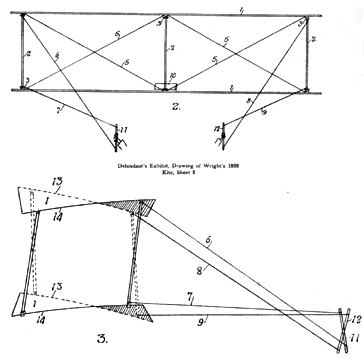
\includegraphics[width=0.8 \textwidth]{state-of-the-art/WrightBrothers1899Kite}
  \caption[Wright Brothers 1899 kite]{Wright 1899 kite: front and side views, with control sticks. Wing-warping is shown in lower view. \cite{Wright}}\label{fig:Wright}
\end{figure}

%Why to used them?
On conventional aircraft, the need to modify the airflow around the airfoil at different flight conditions is achieve through discrete hinged mechanics such as flaps and ailerons. This mechanism perform well in a limited range around the design point while the outside this range, they have a negative influence in the aerodynamics. The necessary discontinuities in the surface bring forward the boundary layer transition from laminar to turbulent regime. Being able to modify the airflow without discontinuities on the airfoil skin would come along with notable reduction in fuel consumption.

%Why now?
New interest has raised in the recent years in aircraft morphing, mainly due to the appearance of new smart materials that allow more efficient mechanical design that do not necessarily incur weight increase \cite{Lloyd2007}. Another reason that is pushing forward new aircraft morphing technologies is that missions today are in need of higher aircraft versatility to decrease operational costs in the commercial aviation field and aim smaller and more distributed targets in the military field. For example, Airbus has recently patented a design of a downwardly foldable wing tip device applicable for a large passenger aircraft \cite{Boye2015}.

%Different morphing projects - \cite{Barbarino}
A general classification of different wing morphing concepts can be seen in Figure \ref{fig:morphingTypes}: planform modification through variation of sweep angle, span or chord; out-of-plane alteration involving twist, dihedral angle and spanwise bending, and airfoil adjustment achieved by modifications of the airfoil chamber and/or thickness. Under this classification, the morphing technology that is the focus of this project is located under the out-of-plane branch and twist modification.
 

\begin{figure}[!htpb]
  \centering
  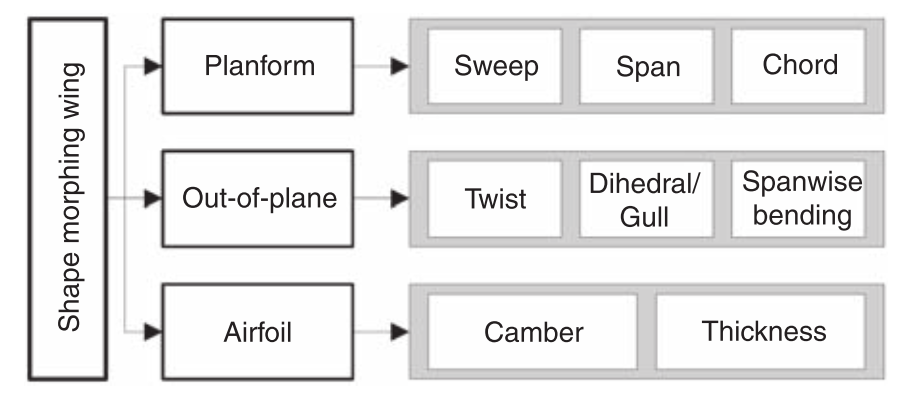
\includegraphics[width=0.8 \textwidth]{state-of-the-art/morphingTypes}
  \caption[Shape morphing wing classification]{Shape morphing wing classification. \cite{Barbarino2011}}\label{fig:morphingTypes}
\end{figure}

%Fundamental idea
Morphing designs may also benefit from geo-metrically flexible structures if the aeroelastic energy from the airstream can be used to activate the shape changing and tabs can maintain the shape using aero-elastic control.

%NASA morphing proyect

\section{Wing twist morphing} \label{sec:twist_state}

In the present section, an analysis of different concepts used to achieve .

The concept of varie the wing twist to modify the airfoil exploits the 
